% This example is meant to be compiled with lualatex or xelatex
% The theme itself also supports pdflatex
\PassOptionsToPackage{unicode}{hyperref}
\documentclass[aspectratio=1610, 9pt]{beamer}

% Load packages you need here
\usepackage{polyglossia}
\setmainlanguage{english}
\setotherlanguages{german}

\usepackage{csquotes}

\usepackage{amsmath}
\usepackage{mathrsfs}
\usepackage{amssymb}
\usepackage{mathtools}
\usepackage{hyperref}
\usepackage{bookmark}
\usepackage{emoji}
\usepackage{tikz}
\usepackage[compat=1.1.0]{tikz-feynman}
\usepackage{appendixnumberbeamer}
\usepackage{color}
\usepackage[most]{tcolorbox}
\tcbset{colback=yellow!10!white, colframe=red!50!black, 
        highlight math style= {enhanced, %<-- needed for the ’remember’ options
            colframe=red,colback=red!10!white,boxsep=0pt}
        }
\usepackage{empheq}
\newcommand*\widefbox[1]{\fcolorbox{tugreen}{white}{\hspace{2em}#1\hspace{2em}}}

\usepackage[
  locale=UK,                   % UK Einstellungen
  separate-uncertainty=true,   % immer Unsicherheit mit \pm
  per-mode=symbol-or-fraction, % / in inline math, fraction in display math
]{siunitx}

\usepackage{graphicx, caption, subcaption}

% load the theme after all packages

\usetheme[
  showtotalframes, % show total number of frames in the footline
  % dark, % optional dark theme, uncomment to use
]{tudo}

% Put settings here, like
\unimathsetup{
  math-style=ISO,
  bold-style=ISO,
  nabla=upright,
  partial=upright,
  mathrm=sym,
}

\usepackage[
  % style=numeric,
  % style=authoryear-ibid,
  % style=verbose,
  doi=false,
  style=phys,
  % sorting=none,
  backend=biber,
  autolang=hyphen,
  articletitle=false,
  chaptertitle=false,
  biblabel=brackets,
  eprint=false,
  pageranges=false,
  doi=false,
  % useauthor=false,
]{biblatex}
% Quellendatenbank
\addbibresource{lit.bib}

\DeclareCiteCommand{\citecustom}
  {\usebibmacro{prenote}}
  {\usebibmacro{citeindex}%
   \printnames{author}%
   \setunit{\labelnamepunct}\newblock
   \printfield{title}%
   \setunit{\addcomma\space}%
   \printfield{eprint}%
   }
  {\multicitedelim}
  {\usebibmacro{postnote}}

\title{BSM seminar talk: Axion models and EFT}
\author{Can Toraman \& Theodor Zies}
\date{04.07.2024}
\institute[Department of physics]{Supervision: Prof. Dr. Gudrun Hiller}
\titlegraphic{
\includegraphics[width=0.8\textwidth]{logos/Axion.jpeg}}

\captionsetup[figure]{labelformat=empty}
\captionsetup[table]{labelformat=empty}


\begin{document}

\begin{frame}
\titlepage
\end{frame}

\begin{frame}{Overview}
  \begin{columns}
    \column{\textwidth}
    \begin{itemize}
      \item Table of contents
      \item Talk based on \citecustom{paper}: "TASI Lectures on the Particle Physics and Astrophysics of Dark Matter"
    \end{itemize}
  \end{columns} 
\end{frame}

\begin{frame}{Standard Model of Elementary Particles}
  \begin{columns}
    \centering
    \column{.5\textwidth}
    \begin{itemize}
      \item Standard Model of Particle Physics (SM) incomplete \\ (e.g. Dark Matter, Dark Energy, Neutrino masses)
      \item Search for New Physics (NP)
      \item Possible new particle candidate: Axions
      \item Axions could solve dark matter and strong CP problem
    \end{itemize}
    \column{.5\textwidth}
    \begin{figure}
    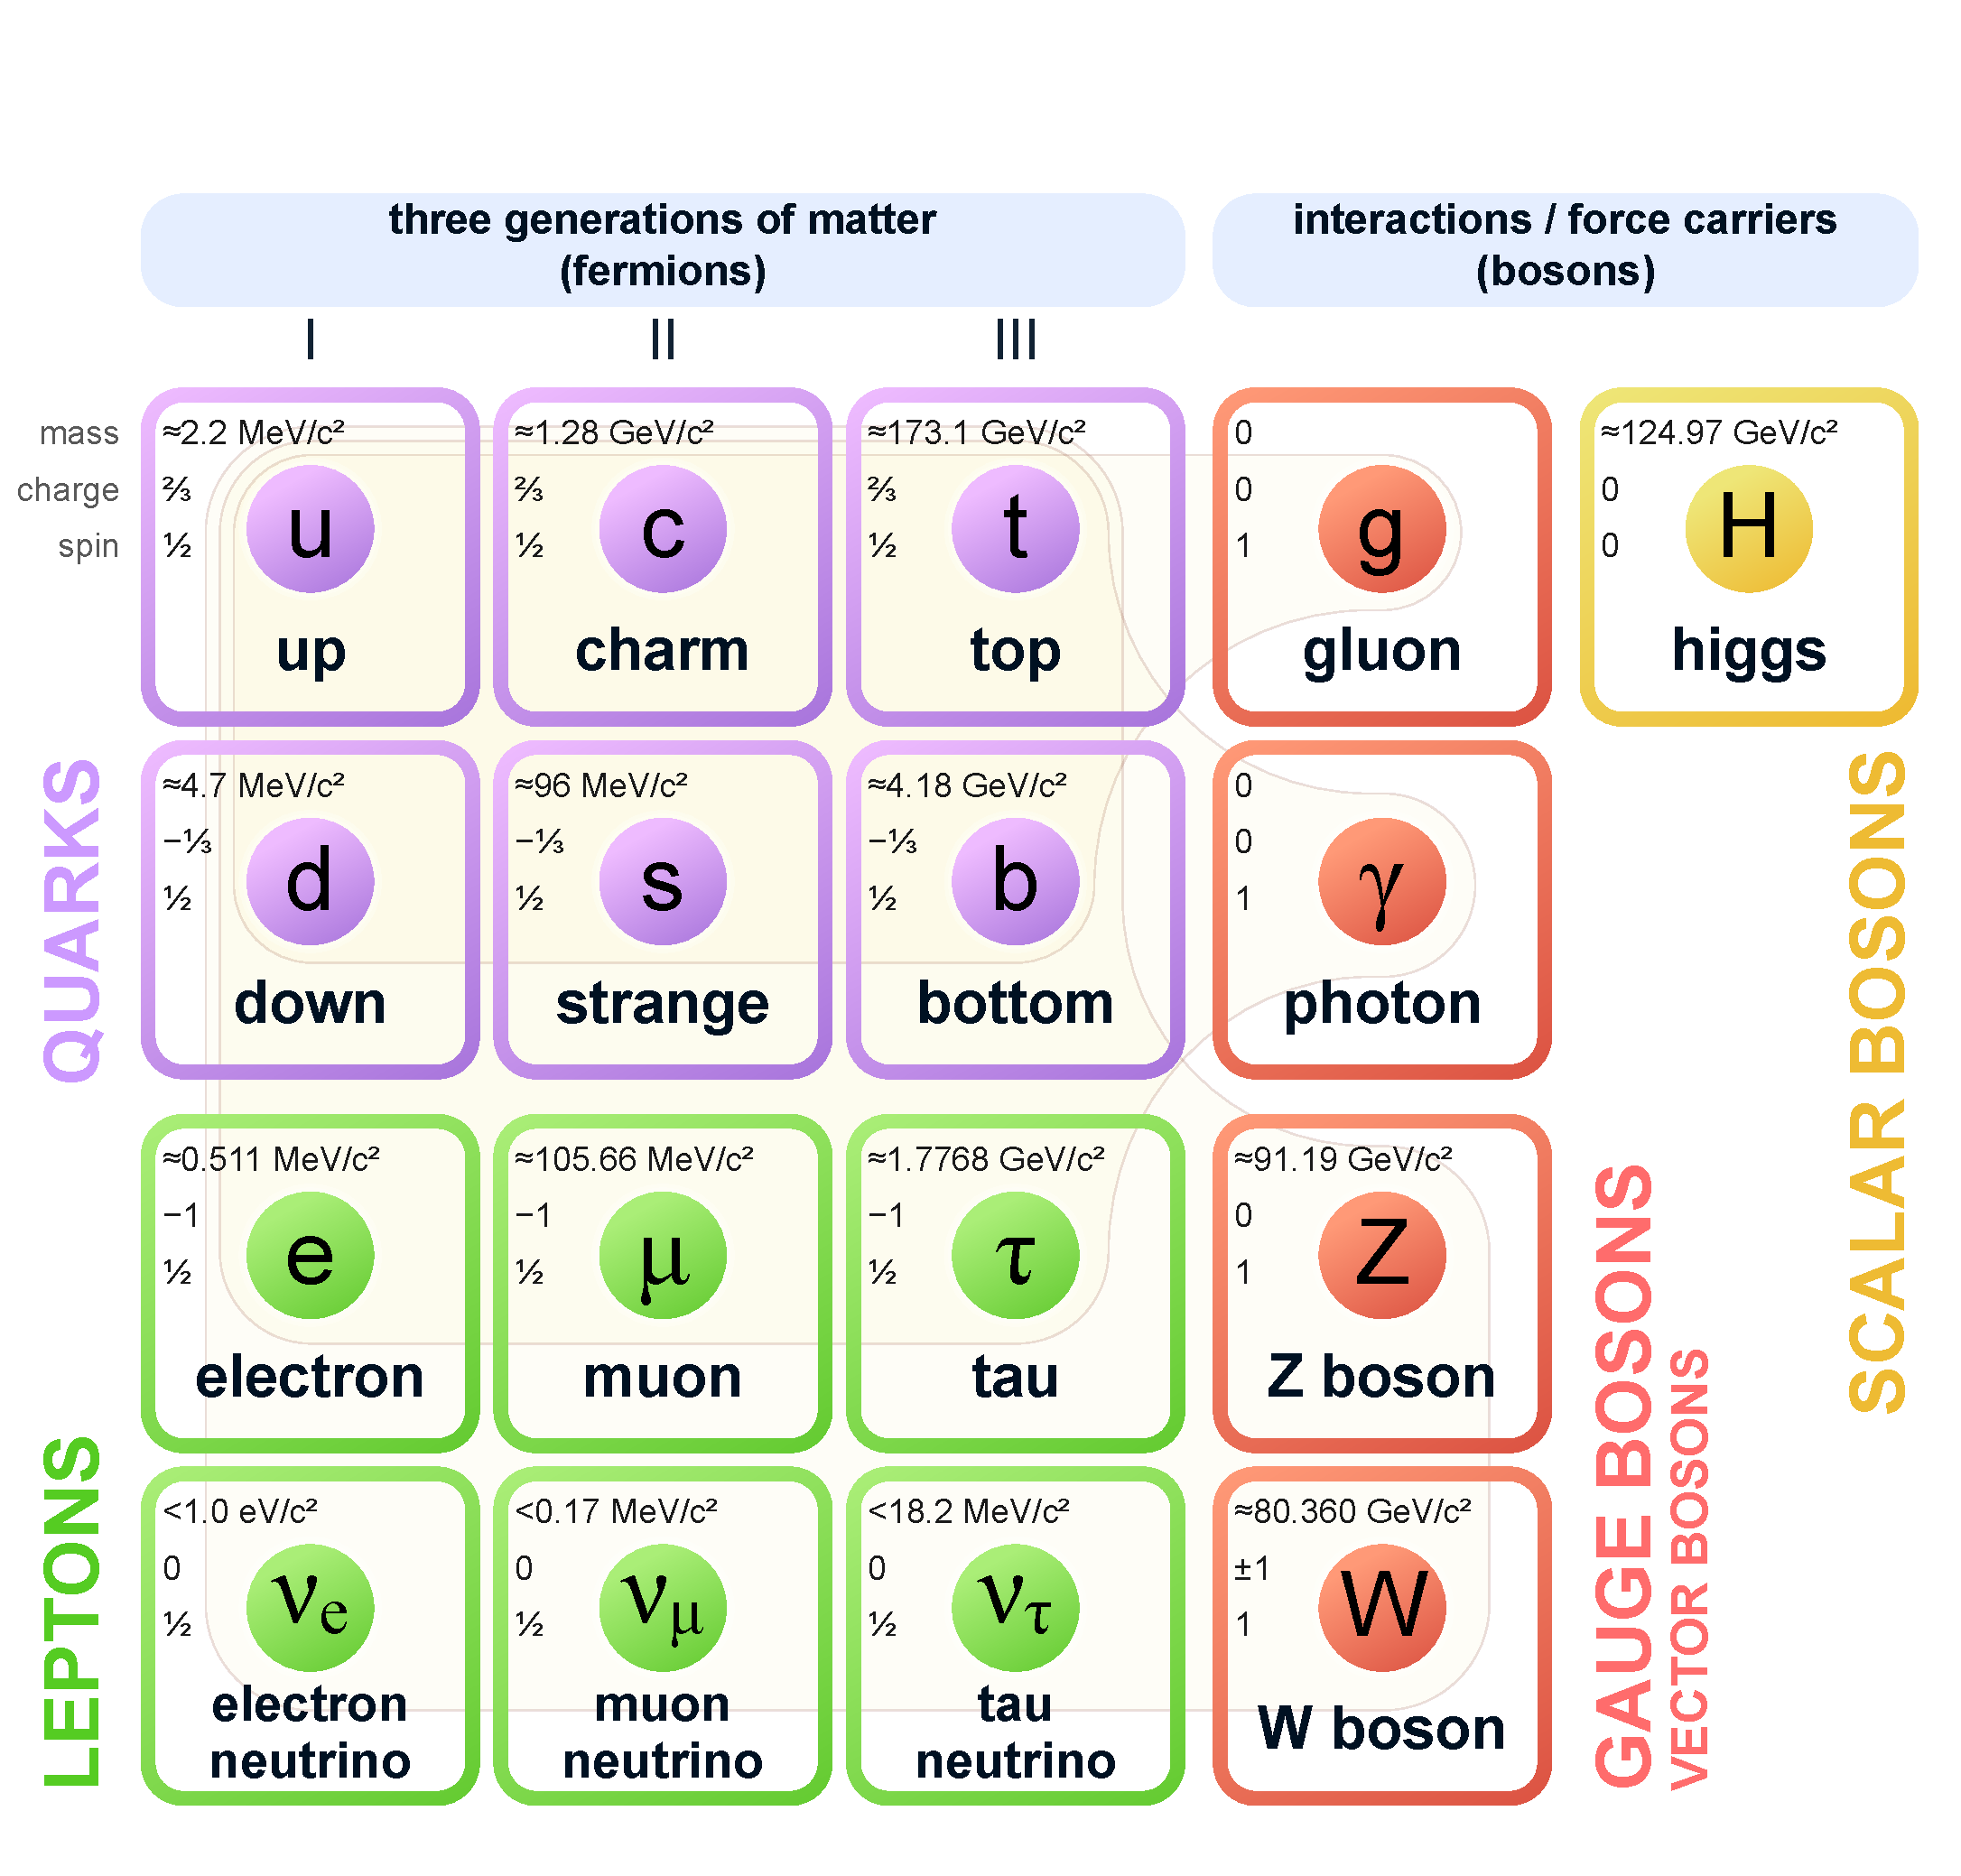
\includegraphics[height=6cm]{images/SM.pdf}
    \caption{\footnotesize \href{https://commons.wikimedia.org/wiki/File:Standard_Model_of_Elementary_Particles.svg}{{[commons.wikimedia.org]}}}
    \end{figure}
  \end{columns} 
\end{frame}

\begin{frame}{Why Axions?}
  \begin{columns}
    \column{.5\textwidth}
    \begin{itemize}
      \item QCD allows for CP violation in SM
      \item Observe CP conservation in strong interaction $\rightarrow$ Strong CP problem
      \item Parameter $\bar{\theta}$ has to be fine tuned to be zero
      \item Physical meaning of $\bar{\theta}$: controls electric dipole moment of neutron
      \item Axions provide a dynamical explanation for $\bar{\theta}=0$
      \item Dark matter is also explainable through axions
    \end{itemize}
    \column{.5\textwidth}
      \begin{figure}
      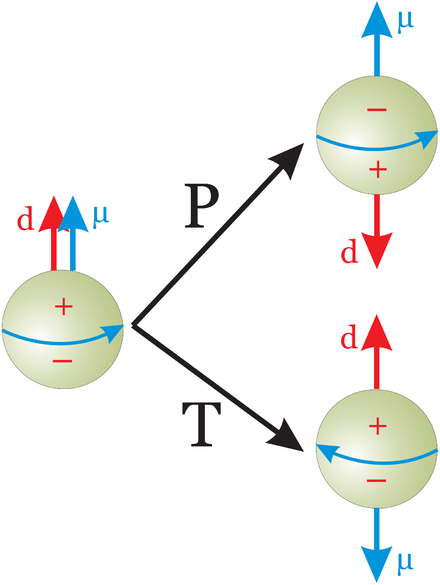
\includegraphics[height=6cm]{images/nEDM.png}
      \caption{\footnotesize \href{https://commons.wikimedia.org/wiki/File:NEDM_P26T_violation.png}{{[commons.wikimedia.org]}}}
      \end{figure}
  \end{columns} 
\end{frame}


\begin{frame}{Effective axion implementation}
  \begin{columns}
    \column{\textwidth}
    \begin{itemize}
      \item Introduce a massless, pseudo-scalar field $a(x)$ that has the dimension-five interaction with QCD:
    \end{itemize}
    \begin{equation*}
      \mathcal{L} \supset \frac{1}{2} \partial_\mu a \partial^\mu a - \frac{g_s^2}{32 \pi^2} \frac{a}{f_a} G^a_{\mu \nu} \tilde{G}^{a \mu \nu}
    \end{equation*}
    \begin{itemize}
      \item $f_a > 10^{9} \, \text{GeV}$ is the UV cut-off of the theory
      \item The QCD axion potential $V(a)$ dynamically sets $\bar{\theta} \rightarrow 0$
    \end{itemize}
    \begin{equation*}
      V(a) = -F_{\pi}^2 m_{\pi}^2 \sqrt{1 - 4 \frac{m_u m_d}{(m_u + m_d)^2} \sin \left( \frac{1}{2} \left( \bar{\theta} + \frac{a}{f_a} \right) \right)^2 }
    \end{equation*}
    \begin{itemize}
      \item Axions aquire a small mass:
    \end{itemize}
    \begin{equation*}
      m_a \approx \frac{F_{\pi} m_{\pi}}{f_a} \approx 6.0 \times 10^{-6} \left( \frac{10^{12} \, \text{GeV}}{f_a} \right) \text{eV}
    \end{equation*}
  \end{columns} 
\end{frame}



\begin{frame}{Axion models}
  \begin{columns}
    \column{\textwidth}
    \begin{itemize}
    \item Many different axion models exist
    \item Goal: Describe how effective axion arises from UV physics
    \end{itemize}
    \begin{enumerate}
      \item Field theory
      \item Extra dimensions, string theory
      \item Axiverse from an EFT perspective
    \end{enumerate}
  \end{columns} 
\end{frame}

\begin{frame}{Field theory axion models}
  \begin{columns}
    \column{\textwidth}
    \begin{itemize}
      \item Axion emerging as pseudo-Goldstone boson of a $U(1)_{\text{PQ}}$ symmetry, known as the Peccei-Quinn (PQ) symmetry
      \item PQ symmetry is spontaneously broken below high scale $f_a$
      \item Introduce complex scalar field $\Phi$ with vacuum expectation value $v_a$:
    \end{itemize}
    \begin{equation*}
      \Phi(x) = \frac{r(x)+v_a}{\sqrt{2}}\exp \left(i\frac{a(x)}{v_a}\right) 
    \end{equation*}
    \begin{itemize}
    \item The PQ Langrangian allows spontaneous symmetry breaking:
    \end{itemize}
    \begin{align*}
      \mathcal{L}_{\Phi} &= \frac{1}{2} \partial_\mu \Phi \partial^\mu \Phi^\dagger - V(\Phi) \\
      & =  {| \partial_\mu \Phi |}^2 - \lambda \left( |\Phi|^2 - \frac{v_a^2}{2} \right)^2
    \end{align*}
    \begin{itemize}
      \item Axion is massless
      \end{itemize}
  \end{columns} 
\end{frame}

\begin{frame}{Kim-Shifman-Vainshtein-Zakharov (KSVZ) model}
  \begin{columns}
    \column{\textwidth}
    \begin{itemize}
      \item Add $N$ identical vector-like fermions $Q_i$, $i=1,2,..,N$
      \item Charges (3, 1, 0) under $SU(3)_c × SU(2)_L × U(1)_Y$ symmetry
      \item Take $\Phi$ to be a SM singlet
      \item Write down the interaction terms between the $Q_i$ and $\Phi$:
    \end{itemize}
    \begin{equation*}
      \mathcal{L}_{\text{int}} = \sum_i \bar{Q}_i i \not{D} Q_i - \sum_i \left( y_i \bar{Q}_i Q_i \Phi + \text{h.c.} \right)
    \end{equation*}
    \begin{itemize}
      \item $y_i$ are Yukawa coupling constants
    \end{itemize}
  \end{columns} 
\end{frame}

\begin{frame}{Arriving at the EFT axion (1/2)}
  \begin{columns}
    \column{\textwidth}
    \begin{itemize}
      \item The full langrangian is invariant if the following symmetries hold:
    \end{itemize}
    \begin{align*}
      \Phi \rightarrow \Phi' &= e^{i \alpha} \Phi \quad U(1)_{\text{PQ}} \,\, \text{symmetry} \\
      Q_i \rightarrow Q_i' &= e^{\frac{i \alpha \gamma_5}{2}} \Phi \quad \text{Anomalous symmetry}
    \end{align*}
    \begin{itemize}
      \item At low energy scales $r(x) \ll v_a$:
    \end{itemize}
    \begin{equation*}
      \Phi(x) \rightarrow \frac{v_a}{\sqrt{2}}\exp \left( i\frac{a(x)}{v_a} \right) 
    \end{equation*}
    \begin{itemize}
      \item Substitute into $\mathcal{L}_{\text{int}}$ and define quark masses $m_i = \frac{y_i v_a}{\sqrt{2}}$:
    \end{itemize}
    \begin{equation*}
      \mathcal{L}_{\text{int}} = \sum_i \bar{Q}_i i \not{D} Q_i - \sum_i \left( m_i \bar{Q}_i Q_i \exp \left( i\frac{a(x)}{v_a} \right) + \text{h.c.} \right)
    \end{equation*}
  \end{columns} 
\end{frame}

\begin{frame}{Arriving at the EFT axion (2/2)}
  \begin{columns}
    \column{\textwidth}
    \begin{itemize}
      \item Apply the axial transformation to the quark fields (anomalous symmetry)
      \item Axion is removed from the interaction langrangian
      \item Following new term is induced:
    \end{itemize}
    \begin{equation*}
      \mathcal{L} \supset \frac{g_s^2}{32\pi^2} \frac{a}{v_a} N G^a_{\mu\nu} \tilde{G}^{a\mu\nu}
    \end{equation*}
    \begin{itemize}
      \item Exactly the dimension-five interaction with QCD if:
    \end{itemize}
    \begin{equation*}
      f_a = \frac{v_a}{N}
    \end{equation*}
    \begin{itemize}
      \item Integer $N$ known as \textit{domain wall number}
      \item Heavy fermion $Q$ is integrated out at the low scale
    \end{itemize}
  \end{columns} 
\end{frame}

\begin{frame}{Problems of the field theory axion}
  \begin{columns}
    \column{.5\textwidth}
    \begin{itemize}
      \item $N>1$ raises cosmological problems in UV completion of the theory
      \item Axion theories face "PQ quality problem"
      \item PQ symmetry needs to be a really good symmetry
      \item Problematic in picture of quantum gravity
      \item Quantum gravity not expected to conserve global symmetries \rightarrow black holes
    \end{itemize}
    \column{.5\textwidth}
    \begin{figure}
    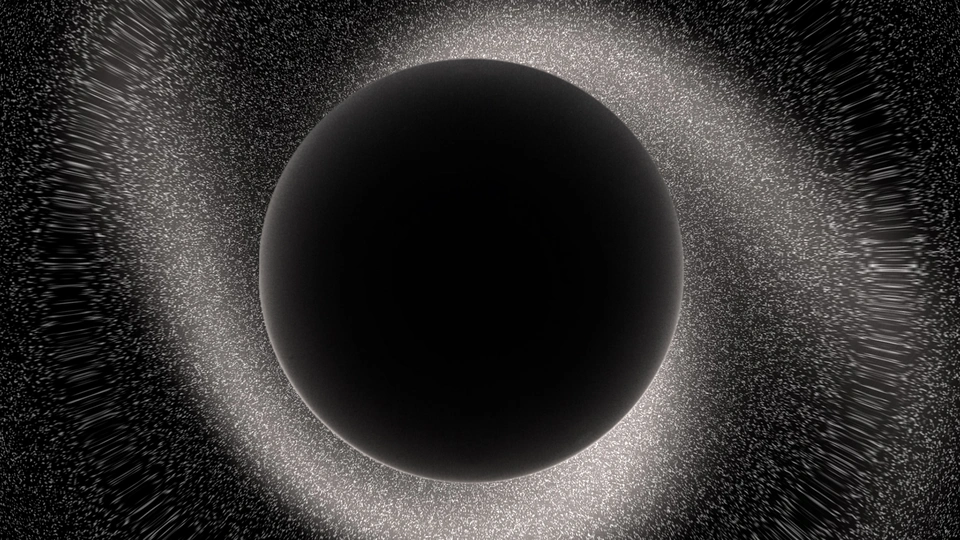
\includegraphics[height=4cm]{images/hole.png}
    \caption{\footnotesize \href{https://www.theatlantic.com/science/archive/2021/03/black-hole-cygnus-suprise/618049/}{{[theatlantic.com]}}}
    \end{figure}
  \end{columns}
\end{frame}

\begin{frame}{Breaking the PQ symmetry}
  \begin{columns}
    \column{\textwidth}
    \begin{itemize}
      \item Black holes should violate the global symmetry
      \item Break the symmetry at the planck scale $m_{\text{pl}}$:
    \end{itemize}
    \begin{equation*}
      \mathcal{L} \supset \lambda \frac{|\Phi|^{2n} \Phi^m}{m_{\text{pl}}^{2n+m-4}} + \text{h.c.}
    \end{equation*}
    \begin{itemize}
      \item $n$ and $m$ are integers, $\lambda$ is dimensionless coupling constant
      \item New relation with $\bar{\theta}$ arises:
    \end{itemize}
    \begin{equation*}
      \langle a \rangle + \bar{\theta} \sim \lambda \left( \frac{f_a}{m_{\text{pl}}} \right)^{2n+m} \left( \frac{m_{\text{pl}}}{\Lambda_{\text{QCD}}} \right)^4
    \end{equation*}
    \begin{itemize}
      \item $n$ and $m$ have to be very large or $\lambda$ really small
      \item New fine tuning problem, because otherwise $\bar{\theta}$ is not close to zero
    \end{itemize}
  \end{columns} 
\end{frame}


\begin{frame}{Axions from string theory}
  \begin{columns}
    \column{\textwidth}
    \begin{itemize}
      \item Equations etc
    \end{itemize}
  \end{columns} 
\end{frame}

\begin{frame}{Axiverse from an EFT perspective}
  \begin{columns}
    \column{\textwidth}
    \begin{itemize}
      \item Equations etc
    \end{itemize}
  \end{columns} 
\end{frame}

\end{document}